\externaldocument{capitulo03}

\chapter{\hspace*{3pt} Modelo Conceitual}
\label{chap:modeloConceitual}

Modelo é a representação abstrata e simplificada de um sistema real, com a qual se pode explicar ou testar o seu comportamento em seu todo ou em partes \citep{castro:2010.abordagem, cougo:1997.modelagem}.

Dada a complexidade do mundo em sua totalidade e necessidade do homem em entender a realidade, os modelos possuem a função de simplificar a realidade de maneira inteligível, permitindo ao homem apreendê-lo e compreendê-lo em suas partes essenciais para um determinado domínio ou campo de estudo \citep{almeida:2006.modelo, dodebei:2002.tesauro}.

O processo de modelar demanda o deslocamento do mundo dos fenômenos para um espaço de representação. Modelar o mundo e representar o conhecimento disponível requer entendimento dos papéis que tal representação pode desempenhar \citep{campos:2004.modelizacao}.

Os modelos são entidades importantes e integram as raízes do método científico: “[...] todas as teorias e modelos científicos são aproximações da verdadeira natureza das coisas; o erro envolvido na aproximação é não raro, suficientemente pequeno para tornar significativa essa aproximação” (\citealp[p.83]{capra:1983.tao} \textit{apud} \citealp{almeida:2006.modelo}).

Os modelos conceituais têm por objetivo desenvolver uma descrição coerente do significado dos dados, satisfazendo nossas necessidades de conhecimento e conceituação sobre determinado domínio, antecipando ou substituindo a existência de uma realidade qualquer \citep{higuchi:2012.representaccao}.

Os modelos devem, portanto, servir como fontes de referencia, quando dúvidas acerca do domínio surgirem, e como um repositório de conhecimento comum, auxiliando a comunicação, o aprendizado e o seu reuso em um nível mais alto de abstração. (\citealp{arango:1994.domain} \textit{apud} \citealp{guizzardi:2000.desenvolvimento}). 

A perspectiva cognitiva é adotada por vários modelos na Ciência da Informação: modelos de representação de usuários e suas necessidades, modelos de representação de estratégia de busca, modelos de representação de documentos. Os primeiros modelam situações problemáticas dos usuários frente a sistemas de informação; os segundos examinam os aspectos cognitivos do processo de transferência de informação entre o usuário e o especialista da informação; e os últimos podem ser modelos mentais do usuário, segundo a perspectiva do sistema, ou modelos conceituais apresentados ao usuário pelo projetista do sistema (\citealp{sayao:2001.modelos} \textit{apud} \citealp{almeida:2006.modelo}).

Metamodelos distintos são utilizados para a representação de Modelos Conceituais, porém o processo de modelagem é anterior a sua representação. Com o intuito de entender como modeladores distintos, reagem a tarefa de representar, através de um modelo, o seu entendimento acerca de um domínio e como o ato de modelar desperta sua próprias experiências para que possam expressar os conceitos, realizamos um estudo de caso.

\section{\hspace*{3pt} Primeiros Estudos}
\label{sec:estudos}

Para esse estudo, foram convidados cinco analistas de sistemas de informação, com experiência, acadêmica ou profissional, na elaboração de modelos conceituais. O perfil foi definido buscando, casos que pudessem exemplificar entre analistas os extremos entre suas experiências \citep{wainer:2007.metodos}.

Nossa questão norteadora foi a de saber \textbf{como diferentes pessoas interpretam um contexto e como suas experiências pessoais podem se refletir sobre sua representação acerca desse mesmo contexto?}

Os dados foram coletados através da gravação do processo de modelagem e os participantes passaram por uma entrevista ao final do processo.

Como tarefa, os participantes deveriam analisar o contexto de uma rede de cinemas, e baseados em suas experiências e conhecimentos sobre a área de negócios e atuação de cinemas em geral, construir um modelo que fosse capaz de representar seu conhecimento sobre as atividades deste contexto e suas relações existentes. Foi sugerido que os participantes considerassem toda atividade ou processos que julgassem pertinentes ao contexto e, se possível, vislumbrassem a expansão do negócio (novas salas, novos cinemas, vendas on-line, tudo que julgassem necessário de acordo com sua experiência).

Para a representação do modelo, o participante poderia utilizar a linguagem que ele se sentisse mais a vontade ou tivesse maior domínio (ER, UML, OntoUML, OWL, etc.)

Os relatos abaixo, foram frutos das entrevistas realizadas com os participantes.

Sobre o domínio, todos os participantes relataram nunca terem precisado criar quaisquer tipos de modelos ou descrições explicitas sobre o contexto, embora tenham o hábito de frequentar cinemas ao menos uma vez ao mês, em média. Isso lhes garantiu, segundo a maioria dos relatos uma visão superficial do  contexto. Um dos participantes ressaltou que a correta representação de um domínio, depende da aprofundação de estudos acerca de seu funcionamento.

Embora tenham alegado um conhecimento parco acerca do domínio, quando indagados, nenhum deles relatou quaisquer problemas para efetuar o modelo. O que sugere que as características dominadas e consolidadas como unidade de conhecimento, permitiram gerar conceitos determinados e falar sobre o contexto com propriedade, de acordo com suas experiências e vivências.

Um ponto a destacar, diz respeito a suas concepções acerca do domínio. Apesar de nenhum relatar dificuldade, a apresentação da tarefa, propositalmente, descrevia o domínio com um conceito geral: ``cinema''. A ideia era despertar a maior quantidade de conceitos subalternos possíveis que os participantes fossem capazes de acessar. Porém todos sentiram a necessidade de questionar quais abordagens deveriam seguir para suas representações. 

Neste aspecto, podemos perceber que a contextualização está fortemente associada a maneira como definimos nossos conceitos. Na falta de uma contexto explícito, todos optaram por seguir a contextualização do usuário, isto é, representar o seu próprio entendimento, os aspectos que estavam acostumados a interagir e da maneira como o faziam.

A experiência pessoal, neste sentido, foi bastante importante. Embora todos reconheçam de alguma maneira que é preciso fazer a compra do ingresso, descrever esse processo através do modelo trouxe dificuldades. Alguns participantes, relataram que pensar sobre essa questão exigiu uma maior dedicação, em partes por possuírem regras que não dominavam e em partes por agregarem novos conceitos ao contexto, como por exemplo: o processo de compra \textit{on-line}.

Os participantes que já haviam, de alguma maneira, lidado com questões semelhantes, conseguiram representar essa tarefa traçando um paralelo entre tarefas ou mesmo domínios semelhantes. Destacamos aqui aqueles com maior tempo de atuação no mercado de trabalho.

A formação acadêmica dos participantes não foi um fator que representasse desvio na analise, visto que mostrou-se bastante homogênea, apenas um dos entrevistados havia feito segundo grau com formação técnica, e todos possuíam ou estavam na pós-graduação, além de possuírem domínio acerca do metamodelo UML, ou outro equivalente, e já terem trabalhado com bancos de dados, ao menos em algum grau. Convém ressaltar que a utilização da UML, como forma de representar o domínio, não foi uma escolha unânime.

\subsection{\hspace*{3pt} Descrições dos Processos para Modelagem}
\label{sec:descricoes_modelos}

Descreveremos de maneira mais detalhada possível, como se sucedeu a execução das tarefas por cada um dos participantes, de maneira a tentar demonstrar passo a passo, como exteriorizaram o seu conhecimento acerca do domínio. Em alguns casos, foi possível perceber que alguns símbolos, deram lugar a outros, conforme a modelagem avançava, em outros casos, que após a inserção de um determinado símbolo, outros conceitos eram alcançados, em seguida.

\subsubsection{\hspace*{3pt} Participante 001}
\label{sec:participante_001}

Ao iniciar a tarefa, participante utilizou o MySQL Workbench para lhe auxiliar, optando por uma linguagem UML para representar seu modelo conceitual. Ao ser apresentado à tarefa, o participante questionou que tipo de visão deveria priorizar, ao que foi respondido que deveria seguir sua própria experiência e interações com o contexto.

O participante adotou uma abordagem \textit{top-down}, partindo de agrupamentos mais amplos, nomeados com conceitos gerais e pouco a pouco adicionando os conceitos mais específicos. Pôde-se observar que o participante possui um forte senso de organização, preocupando-se em criar previamente, com a ferramenta adotada, espaços - denominados \textit{layers} na ferramenta - que representavam os conceitos gerais e que iriam servir como agrupadores para os conceitos mais específicos. 

Por ser o contexto, uma rede de cinemas, o participante 001 entendeu que o conceito principal deste era \textbf{FILME}, sendo esta a primeira entidade adicionada ao seu modelo. O participante rapidamente identificou três características relacionadas ao conceito filme: \textit{id}, \textit{nome} e \textit{categoria}. Por estar utilizando uma abordagem de banco de dados, a teoria sugere que para evitar duplicidade de informação na armazenagem de dados, todo dado deve ter um identificador único \citep{heuser:2001.projeto, machado:2009.projeto}; que foi representado nesta modelagem como id, sendo então adicionado como uma característica ao conceito de filme, assim como nome. O conceito de nome, sendo adicionado como propriedade de filme, sugere uma intensão específica, na qual um nome está associado única e exclusivamente a um filme, embora o conceito nome possa ter extensão ao se referir ao grupo de todos os nomes possíveis atribuídos a objetos e indivíduos \citep{dahlberg:1978.fundamentos}. Por fim, o participante entendeu que o conceito \textbf{CATEGORIA}, embora fosse uma propriedade de filmes, consistia em uma relação na qual uma mesma categoria de filmes poderia estar associada a diferentes filmes, gerando por esse motivo uma nova entidade. Como propriedades dessa entidade, foram encontrados \textit{id} e \textbf{nome}.

O participante nomeou o \textit{layer} que continha essas duas entidades como FILMES, entendendo que FILME é um agrupamento categorial que engloba os conceitos de Filmes e Categorias.
 
Dando prosseguimento em sua modelagem, o participante nomeou o segundo \textit{layer} como \textbf{CINEMA}, sugerindo que todos os conceitos que fizerem parte desse agrupamento categorial serão inseridos neste espaço. Para esse \textit{layer}, encontrou de imediato o conceito \textbf{SALAS}, cujas propriedades identificadas foram: \textit{id}, \textit{nome} e \textit{lotacao}.

O terceiro \textit{layer} foi considerado o agrupamento categorial de todos os conceitos envolvidos com vendas e por esse motivo, o participante o nomeou como PDV (Ponto de Venda). 

O primeiro conceito encontrado nesse agrupamento foi o de \textbf{VENDAS}. Essa entidade continha como características os conceitos de \textit{id} e \textit{produto}. Sendo produto, um conceito que substituiu seus análogos nas outras tabelas, conhecidos como nome. Produto sugere a existência de um agrupamento intermediário entre vendas e nome, um conjunto formado por outros conceitos, ainda não analisados, cujo conceito nome está contido.

O segundo conceito pertencente a esse agrupamento categorial, foi de \textbf{INGRESSO}, sugerindo que o participante faz uma distinção entre os tipos de compras que se pode fazer em um cinema. Como propriedade, foram encontrados \textit{id} e filme, sendo este último imediatamente substituído por produto, e por fim, por \textit{venda}. Sugerindo que esse conceito se relaciona com o conceito de venda, pertencendo a este, mas sendo importante para o contexto a ponto de estar em uma tabela a parte.

No quarto \textit{layer}, chamado de marktplace, o último dos quatros criados inicialmente, foi inserido o conceito de \textbf{HORARIOS}, cujas propriedades adicionadas foram \textit{id}, \textit{filme}, \textit{sala}, \textit{horario}, onde, filme se relaciona com o conceito FILME, através da relação \textit{horario-filme}. Sala se relaciona com o conceito SALAS, através da relação \textit{horario-sala}.

Outro conceito adicionado a essa agrupamento foi o de \textbf{PRODUTO}. Observou-se que o participante demorou aproximadamente 25 segundos decidindo se esse conceito deveria pertencer ou não ao agrupamento, e a identificação de suas propriedades, pareceram gerar hesitação. Por fim, as propriedades adicionadas foram: \textit{id}, \textit{horario} e \textit{valor}. A relação entre \textbf{PRODUTO} e \textbf{HORARIOS}, pareceu gerar igualmente indecisão, mas no fim, o participante optou por adicionar a relação \textit{produto-horario}. Na sequência, a relação entre os conceitos \textbf{PRODUTO} e \textbf{VENDA}, fora estabelecida pela relação \textit{venda-produto}. 

A relação entre INGRESSO e VENDA, denominada \textit{ingresso-venda}, apresentou demora quanto sua decisão de inserção.

A partir deste ponto, o participante pareceu procurar de maneira mais cuidadosa propriedades e relações que pudessem fazer parte dessa representação. Novos conceitos, fossem com grande extensão ou intensão, não pareceram estar mais tão evidentes ao participante quanto os primeiros.

Uma análise mais cuidadosa dos conceitos já inseridos e em suas relações, revelou mais duas propriedades, para o conceito VENDA, a saber: \textit{identificador} e \textit{status}. E mais uma propriedade para o conceito INGRESSO, \textit{identificador}. 

Após mais alguns segundos analisando o fluxo possível para execução do processo de compra de ingressos e produtos, o participante julgou necessária a presença de um novo conceito no grupamento PDV. Esse conceito foi identificado como \textbf{OPERADOR}, e lhe foram atribuídas as seguintes propriedades: \textit{id} e \textit{funcionario}. No primeiro momento, funcionário foi definido de forma que sugeria a futura inserção de um conceito FUNCIONARIO que teria relação com o conceito operador, novamente trazendo a ideia de hierarquização entre os conceitos, onde o conceito operador estaria incluído no conceito funcionário.

A presença do conceito \textbf{OPERADOR} se refletiu na necessidade de edição do conceito \textbf{VENDAS}, para a inserção de uma nova relação, denominada \textit{venda-operador}. No grupamento cinema, o participante adicionou o conceito \textbf{PESSOA}, optando por um conceito geral para sua representação, lhe atribuindo as propriedades \textit{id} e \textit{nome}. A partir deste conceito com extensão geral, traçou a relação com o conceito \textbf{OPERADOR}, nomeando como \textbf{operador-pessoa}.

Somente após 8 minutos de observação, o participante adicionou uma nova propriedade ao conceito \textbf{PRODUTO}, cadeira e um novo conceito, desta vez um sendo originado pela ideia de relação entre \textit{venda-produto}. Esse conceito originou a tabela homônima, cujas propriedades definidas foram: \textit{id}, \textit{venda} e \textit{produto}. Esse conceito mantém, como nome sugere, relação com o conceito \textbf{VENDA}, através da relação venda e com o conceito \textbf{PRODUTO}, através da relação produto. Desta forma, o participante descartou a relação\textit{ venda-produto} previamente estabelecida.

No conceito \textbf{INGRESSO}, a propriedade utilizada foi acrescida, sugerindo a ideia de que um ingresso pode ou não ter sido utilizado, após sua aquisição e finalizando o modelo do usuário, que utilizou mais 6 minutos para alguns ajustes de apresentação e organização, totalizando aproximadamente 40 minutos para execução da tarefa.

A Figura \ref{fig:Modelo_000_Marlucio_Barbosa}, representa o modelo gerado pelo pelo participante 001 ao término da tarefa.

\begin{figure}[!ht]
    \centering
    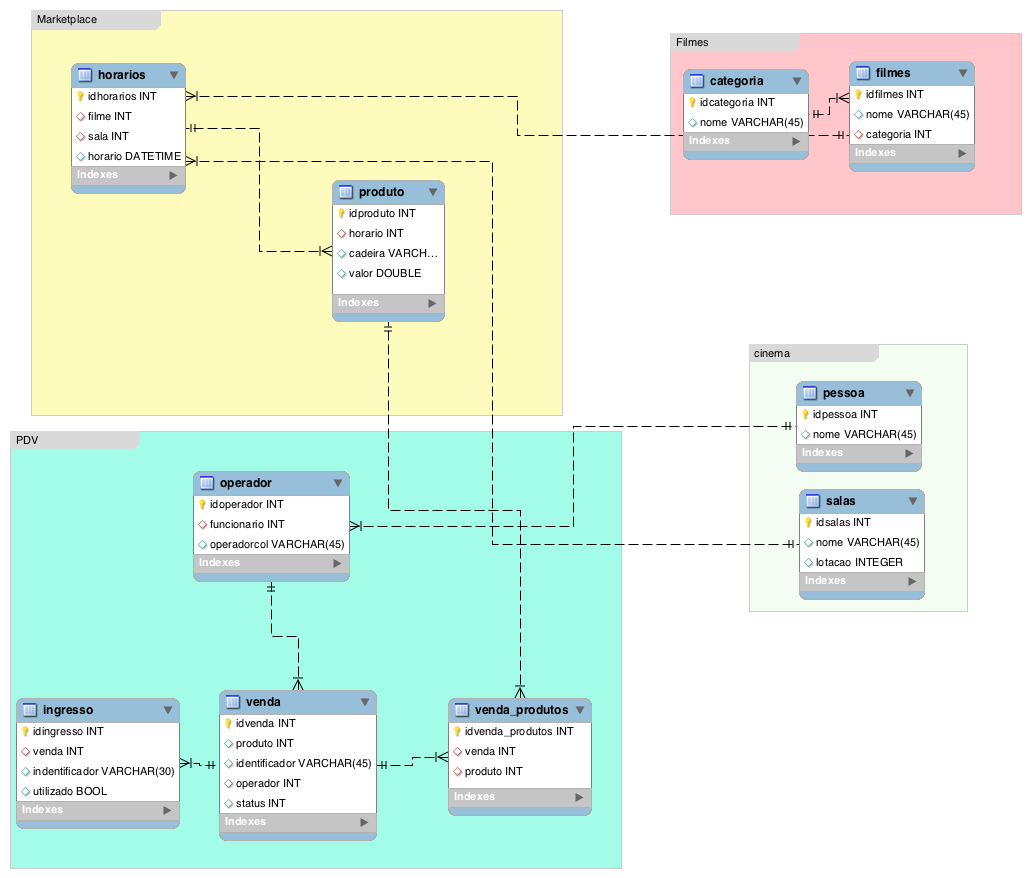
\includegraphics[width=\textwidth]{imagens/Modelo_000_Marlucio_Barbosa.png}
    \caption{Modelo Gerado pelo Participante 001}
    \label{fig:Modelo_000_Marlucio_Barbosa}
\end{figure}

\subsubsection{\hspace*{3pt} Participante 002}
\label{sec:participante_002}

O participante 002 ao ser apresentado ao contexto e a tarefa de representá-lo, pontuou algumas dúvidas acerca desta. O contexto, embora definisse o domínio, carecia de uma visão mais focada que guiasse o participante na direção de uma representação mais específica. Outra dúvida fora sobre a maneira que ele poderia representar o contexto, isto é, que ferramentas ou linguagens poderia se valer para a execução da tarefa.

Fora explicado ao participante que o mesmo deveria tomar as circunstâncias que lhe fossem mais comuns para a representação do contexto e poderia se valer de qualquer linguagem que lhe parecesse mais simples ou detivesse maior experiência de uso. Tendo esclarecido estas questões, o participante optou por utilizar a linguagem E-R, disponibilizada em uma ferramenta web para executar seu modelo.

Seguindo as orientações, o participante definiu primeiro todas as entidades que ele julgou pertinentes ao contexto na seguinte ordem: \textbf{GRUPO}, \textbf{FILIAL}, \textbf{SALA}, \textbf{LOCALIZACAO}, \textbf{SERVICO}, \textbf{FUNCIONARIO}, \textbf{FILME}, \textbf{SESSAO} e \textbf{DISTRIBUIDORA}.

Sua abordagem seguiu a visão \textit{top-down}, onde a entidade mais geral, o grupo que representa todas as salas de cinema, foi a primeira a ser definida, e cada conceito pertencente ao primeiro, fora definido um após o outro.

Após determinar todas as entidades, o participante 002 representou cada uma das relações que as entidades possuíam umas com as outras, de acordo com a sequência: \textbf{GRUPO} se relaciona com \textbf{FILIAL}, \textbf{FILIAL} com \textbf{FUNCIONARIO} e com \textbf{SALA}, \textbf{SALA} por sua vez se relaciona com \textbf{SESSAO} e \textbf{LOCALIZACAO}. Neste ponto, o participante ficou confuso quanto ao tipo de relacionamento que \textbf{SALA} manteria com \textbf{LOCALIZACAO}. Dando continuidade aos relacionamentos, o participante 002 definiu a relação entre \textbf{SESSAO} e \textbf{FILME}, \textbf{FILME} com \textbf{DISTRIBUIDORA} e \textbf{LOCALIZACAO} com \textbf{SERVICO}. 

O participante 002 precisou definir ainda as seguintes entidades \textbf{INGRESSO},  \textbf{CANAL DE VENDA} e \textbf{CONTRATO}, traçando a relação de \textbf{SESSAO} com \textbf{INGRESSO}, \textbf{INGRESSO} com \textbf{CANAL DE VENDA}, \textbf{GRUPO} com \textbf{CONTRATO}, \textbf{CONTRATO} com \textbf{DISTRIBUIDORA}.

Neste ponto, mais uma entidade precisou ser definida, \textbf{USUARIO ON LINE}, que foi relacionada com \textbf{INGRESSO}, gerando novamente dúvidas sobre o tipo de relacionamento que manteriam uma com a outra.

Como última etapa do processo de modelagem, o participante 002 definiu as características que cada entidade da seguinte maneira:

\textbf{GRUPO} (\textit{sede}, \textit{marca}, \sout{\textit{empresa}} ,\textit{cnpj}); \textbf{CONTRATO} (\textit{valor}, \textit{vigencia}, \textit{logistica}); \textbf{FILIAL} (\textit{cnpj}, \textit{responsavel}); \textbf{FUNCIONARIO} (\textit{nome}, \textit{cpf}, \textit{salario}, \textit{funcao}, \textit{cargo}); \textbf{LOCALIZACAO} ( \textit{shopping}, \textit{endereço}); \textbf{SALA} (\textit{mapa de cadeiras}, \textit{código}, \textit{3d}, \textit{imax}, \textit{conforto premium}); \textbf{DISTRIBUIDORA} (\textit{responsavel}, \textit{cnpj}, \textit{contato}); \textbf{FILME} (\textit{titulo}, \textit{classificacao}, \textit{descricao}, \textit{midia}, \textit{trailer}); \textbf{SESSAO} ( \textit{horario}, \textit{dublado/legendado}, \textit{3D}); \textbf{SERVICO} (\textit{pipoca}, \textit{promocoes}, \textit{bebida}, \textit{doces}, \textit{valor}); \textbf{INGRESSO} (\textit{beneficio meia?}, \textit{valor inteira}, \textit{data compra} \textit{forma de pagamento}*); \textbf{CANAL DE VENDA} (\textit{internet}, \textit{guiche}); \textbf{USUARIO ON LINE} (\textit{id}, \textit{nome}).

Pode se observar, porém, que na entidade \textbf{GRUPO}, o participante teve dúvidas acerca de que símbolo utilizar para representar o conceito do nome do grupo da empresa. A palavra riscada, representa o signo preterido em favor do signo escolhido, marca. A características \textit{forma de pagamento}, marcada com asterisco (*), somente foi acrescentada após as definições das características de \textbf{Canal de Vendas}, evidenciando que um conceito conectou ao outro.

A preocupação do participante 002 em demonstrar informações como distribuidora, classificação, tipo de mídia, se a cópia é dublada ou legendada, por exemplo. Pode significar uma maior experiência em relação ao contexto apresentado e sua atividade fim. Seu tempo total de execução do modelo foi de aproximadamente 20 minutos.

A Figura \ref{fig:Modelo_000_igor}, representa o modelo gerado pelo pelo participante 002 ao término da tarefa.

\begin{figure}[!ht]
    \centering
    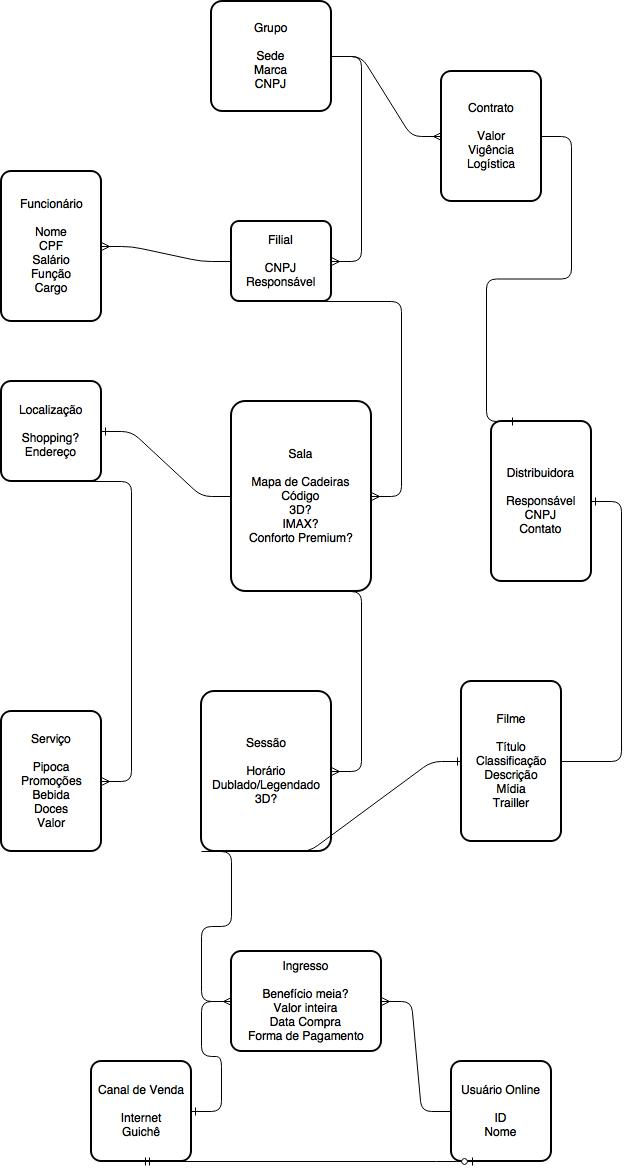
\includegraphics[width=\textwidth, height=\textwidth]{imagens/Modelo_000_Igor.jpg}
    \caption{Modelo Gerado pelo Participante 002}
    \label{fig:Modelo_000_igor}
\end{figure}

\subsubsection{\hspace*{3pt} Participante 003}
\label{sec:participante_003}

O participante 003, também ficou em dúvidas ao ser apresentado à tarefa, questionando como, exatamente, deveria efetuar o modelo. Ao qual foi esclarecido, que assim como constava nas orientações, ele deveria escolher o método para representação que se sentisse mais a vontade e que melhor demonstrasse as particularidades do contexto. Quando questionou sobre que tipo de informações deveria priorizar no modelo, lhe foi solicitado que representasse aquelas que ele julgasse necessárias para demonstrar seu conhecimento sobre a mesma, de maneira clara.

O participante 003 começou sua modelagem às 00:32, optando para executar a tarefa por uma descrição textual das entidades, relacionamentos e propriedades. A primeira entidade descrita por ele, foi \textbf{FILME}, com os atributos básicos \textit{título} e \textit{duração}. Pode-se perceber aqui a associação do conceito cinema, representando o contexto, ao conceito filme, como um conceito mais específico, conforme apresentado por \citep{dahlberg:1978.fundamentos}. A próxima entidade descrita foi \textbf{SALA}, com o atributo \textit{nome}. E depois a entidade CLIENTE, e seus atributos: \textit{nome} e \textit{endereço}, sendo essa última como uma referência para a entidade, ainda vindoura.  A próxima entidade descrita fora \textbf{FUNCIONÁRIO}, possuindo também os atributos \textit{nome} e \textit{endereço}, endereço também como referência.

A entidade \textbf{CINEMA}, foi a quarta entidade a ser descrita e continha os atributos \textit{nome}, \textit{salas} e \textit{endereço}. O símbolo escolhido para representar o conceito sala, estava na forma plural, demonstrando que o participante entende que o conceito cinema, por ser geral, pode conter mais de uma sala, mas apenas um endereço, por esse motivo a falta da forma plural deste último signo. Outro indicador de que as noções hierárquicas estão presentes na modelagem, é o fato que ambos os atributos, entraram como referencias a outras entidades.

A entidade \textbf{SESSÃO}, com os atributos \textit{horário início}, \textit{horário fim}, \textit{preço}, \textit{número total de assentos}, \textit{funcionário responsável}, como referência a entidade \textbf{FUNCIONÁRIO} foi definida. Ainda durante a definição deste conceito, o participante 003 adicionou o símbolo \textit{número}, aos símbolos \textit{total de assentos}, que representavam essa característica. 

\textbf{COMPRA}, com os atributos \textit{cliente}, \textit{sessão}, \textit{número do assento comprado} e \textit{forma de pagamento}, foram foram definidas. o atributo cliente fazendo referência para a entidade \textbf{CLIENTE} e o atributo sessão, fazendo referência para a entidade \textbf{SESSÃO}.

A entidade \textbf{AVALIAÇÃO} com os atributos \textit{compra} fazendo referência a entidade \textbf{COMPRA} e o atributo \textit{nota da avaliação}, foram descritas logo após.

O participante julgou ser preciso esclarecer a necessidade de elaboração de regras para o melhor entendimento do modelo, com por exemplo verificar a quantidade de assentos disponíveis e se um determinado filme ``caberia'' em uma sessão. 

Ao analisar os conceitos definidos, recordou-se que embora prevista, ainda não havia definido a entidade \textbf{ENDEREÇO}, que foi definida com os atributos \textit{rua}, \textit{número} e \textit{etc}. Neste momento, o participante também definiu os atributos \textit{filme} e \textit{sala}, como referências às entidades homônimas, para a entidade \textbf{SESSÃO}, por terem sido definidas em um momento posterior, assinalamos no modelo descrito com asterisco (*).

A execução da tarefa teve seu final às 00:57 e o resultado de seu modelo, por ser textual, está transcrito aqui:

\begin{quote}
FILME\\
	- Título\\
	- Duração (em minutos)\\
SALA\\
	- Nome\\
ClIENTE\\
	- Nome\\
	- Endereço (referência para entidade endereço)\\
FUNCIONÁRIO\\
	- Nome\\
	- Endereço (referência para entidade endereço)\\
CINEMA\\
	- Nome\\
    - Salas (referência para entidade salas)\\
    - endereço (referência para entidade endereço)\\
SESSAO\\
	- Horário início (data/hora)\\
    - Horário fim (data/hora)\\
    - Preço\\
    - Número de assentos disponíveis\\
    - Funcionário responsável (referência para entidade funcionário)\\
    - Filme*\\
    - Sala*\\
COMPRA\\
	- Cliente (referência para entidade cliente)\\
    - Sessão (referência para entidade sessão)\\
    - Número do assento comprado\\
    - Forma de pagamento\\
AVALIAÇÃO \\
	- Compra (referência para entidade compra)\\
	- Nota da avaliação\\
ENDEREÇO \\
	- Rua \\
    - Número \\
    - Etc \\
\end{quote}

\subsubsection{\hspace*{3pt} Participante 004}
\label{sec:participante_004}

Após a explicação da tarefa, o participante em dúvida, questionou acerca da abordagem que deveria seguir para representar o contexto, ao qual foi respondido que deveria seguir aquela que ele julgasse mais adequada para representar o contexto, seguindo sua experiência e interação com o mesmo. 

O participante 004 iniciou sua modelagem às 18:24 e escolheu como ferramenta para auxiliá-lo o programa Astah, no qual optou por fazer um modelo de diagrama de classes. Sua abordagem de modelagem, seguiu a abordagem \textit{top-down} cuja entidade inicial do modelo recebeu o nome do contexto ao qual ele procurava representar, isto é, \textbf{CINEMA}. Na sequência, as entidades \textbf{UNIDADE}, \textbf{ENDERECO} e \textbf{SALA}, e suas relações foram definidas, antes que o participante seguisse na busca de outras entidades.

As entidades definidas na sequência foram: \textbf{ASSENTO}, \textbf{SESSAO} e \textbf{FUNCIONARIO}, assim como suas relações com as entidades já definidas. Nesta avaliação, foi possível notar a influência que a entidade \textbf{SALA}, exerceu na definição das entidades seguintes, assim como nas relações que as novas entidades mantinham com entidade \textbf{SALA}. Percebeu-se que, após a definição da entidade \textbf{FUNCIONARIO}, o participante precisou rememorar suas experiências e comparar com o que estava representando, pois o mesmo não adicionou nenhuma alteração ao modelo por um período longo de tempo, se comparado à performance que estava desenvolvendo até então. Após o período de rememoração, o participante definiu a entidade \textbf{FILME} e a relacionou com a entidade \textbf{SESSAO}, entrando novamente em estado de rememoração.

O próximo passo do participante foi definir os atributos das entidades definidas. Ficou evidente que as características definidas foram àquelas que o participante tinha conhecimento e julgou necessário de acordo com o contexto abordado, por exemplo os atributos \textit{horaInicial} e \textit{horaFinal} para a entidade \textbf{SESSAO}. Durante a definição dos atributos, o participante percebeu a necessidade de uma nova entidade, a qual ele nomeou \textbf{FUNCAO} e a associou as entidades \textbf{UNIDADE} e \textbf{FUNCIONARIO}. 

Duas outras entidades foram definidas em seguida: \textbf{ESTOQUE} e \textbf{PRODUTO}, assim como suas relações. A ordem da definição das entidades, seguindo as experiências demonstradas por \citet{rosch:1975.family}, apontam para a possível ordem que o participante habitualmente interage com o contexto, no qual a \textit{bomboniere} é o ultimo local visitando, antes de entrar na sala para uma sessão de cinema.

O processo de modelagem do participante 004 terminou às 19h, a Figura \ref{fig:Modelo_000_wagner} representa o modelo gerado pela atividade.

\begin{figure}[!ht]
    \centering
    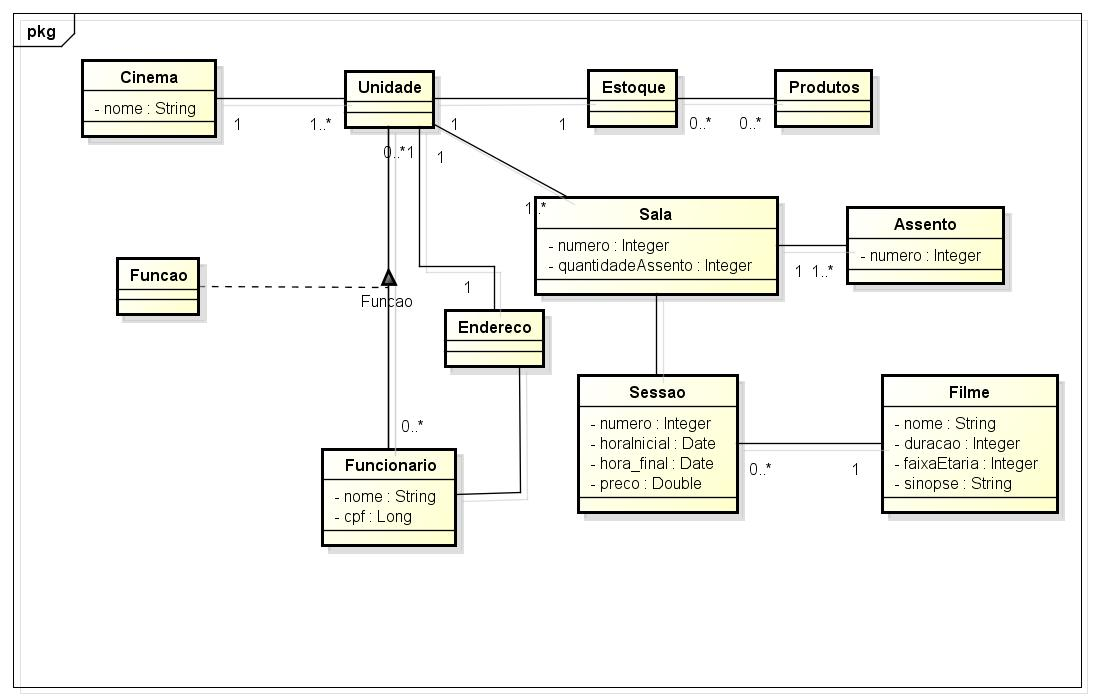
\includegraphics[width=\textwidth, height=\textwidth]{imagens/Modelo_000_Wagner.jpg}
    \caption{Modelo Gerado pelo Participante 004}
    \label{fig:Modelo_000_wagner}
\end{figure}

\subsubsection{\hspace*{3pt} Participante 005}
\label{sec:participante_005}

Ao ser apresentado à tarefa, o participante 005 questionou sobre o tipo de abordagem que deveria seguir. Ao ser indagado sobre a natureza de sua dúvida, o mesmo respondeu que necessitava saber mais sobre o contexto para poder modelá-lo. Ao participante, fora explicado que fazia parte do da pesquisa aferir que abordagem ele escolheria, assim como a maneira que iria implementá-la. Para tal, ele deveria seguir a abordagem que lhe parecesse mais adequada para representar seus conhecimentos sobre o contexto. 

Depois de optar pela linguagem UML e seu diagrama de classes, utilizando papel e lápis, começou a definir as entidades que, segundo ele, representavam sua visão sobre o contexto.

A primeira entidade definida pelo participante fora \textbf{FILME} com os atributos \textit{nome}, \textit{duracao}, \textit{genero}, \textit{produtora} e \textit{atores}. Seguida da entidade \textbf{CINEMA}, possuidora dos atributos \textit{endereco}, \textit{cnpj}, \textit{nome-social} e \textit{telefone}. Percebe-se pelos atributos definidos para a entidade filme, que o participante possui uma afinidade maior com a atividade fim do contexto, se comparado ao demais participantes desta fase, dado o grau de detalhamento que o mesmo dedicou a entidade, e possivelmente a mais importe, pois as demais entidades surgiram em natural associação com as primeiras, por exemplo a entidade \textbf{SESSAO} e seus atributos \textit{data}, \textit{hora} e \textit{numero de identificacao}. 

A entidade \textbf{EMPREGADOS} foi definida em seguida, mantendo ligação com a entidade \textbf{CINEMA}, e para esta entidade o participante definiu os atributos \textit{nome}, \textit{cpf} e \textit{telefone}, determinando a partir desta relação a entidade \textbf{INSCRICAO} com os atributos \textit{numero de identificação} e \textit{sede}.

O processo de modelagem do participante, demorou 4 minutos no total, e a Figura \ref{fig:Modelo_000_modesto} representa o modelo criado.

\begin{figure}[!ht]
    \centering
    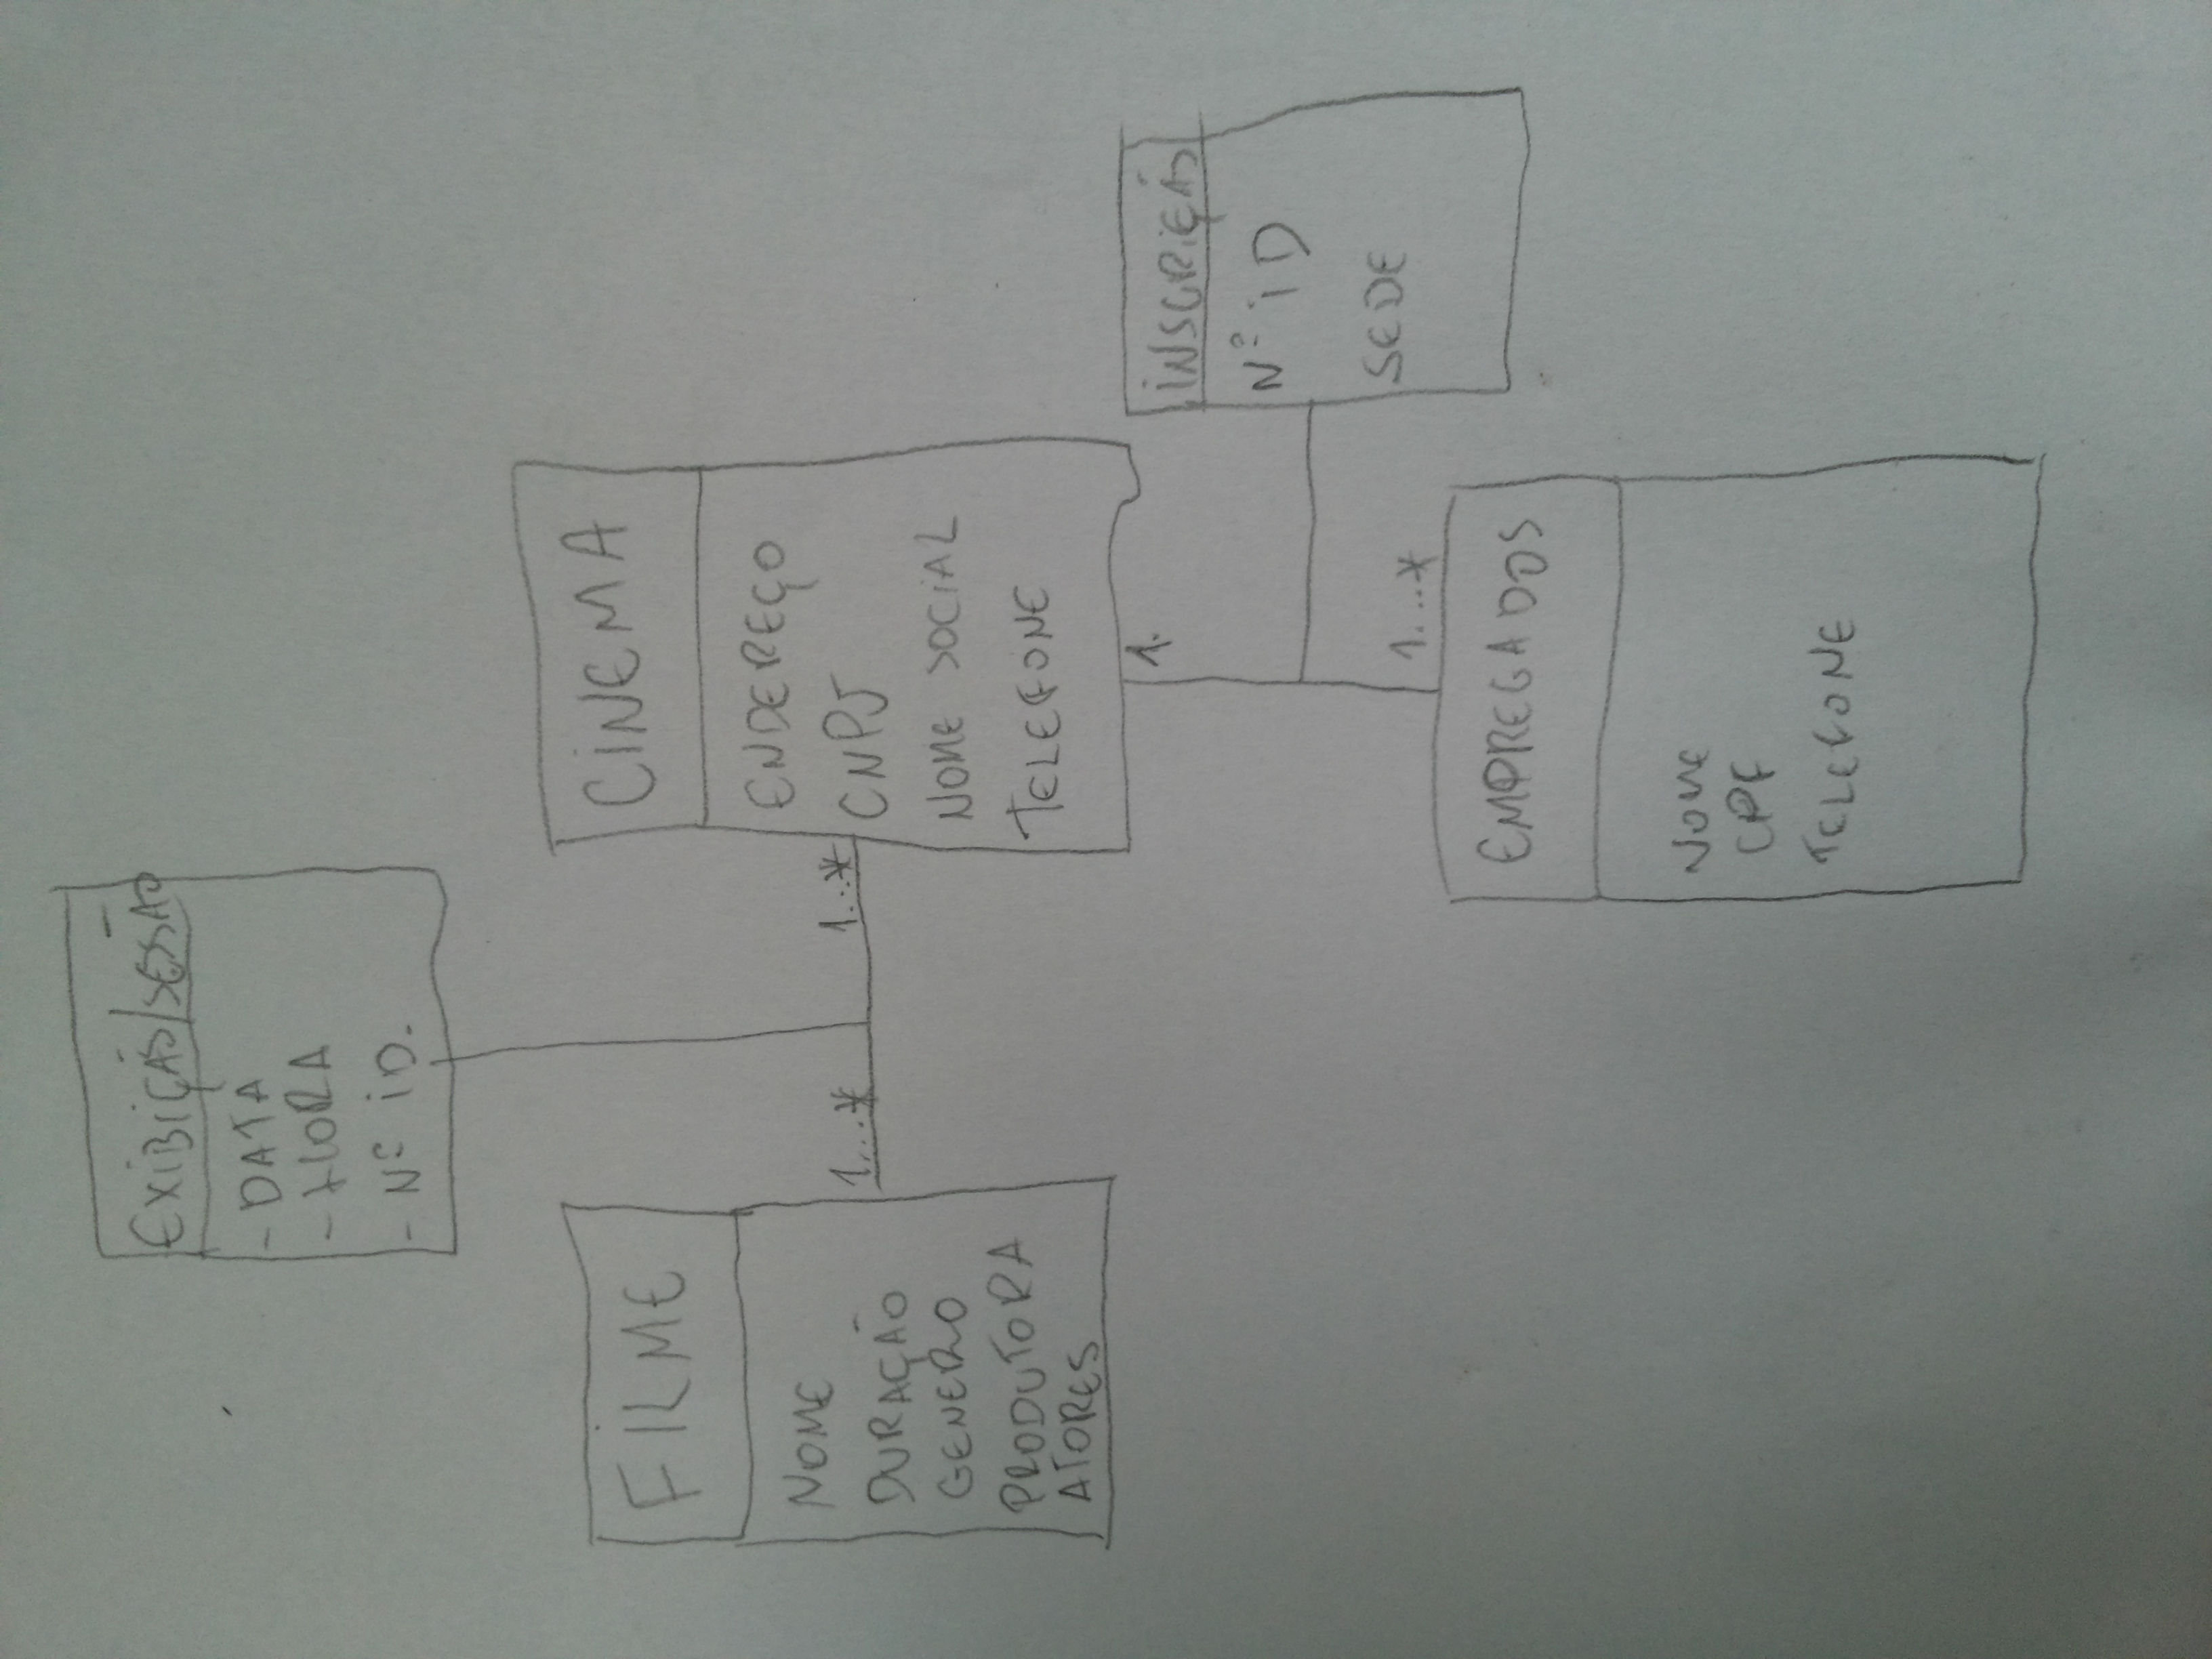
\includegraphics[width=\textwidth, height=\textwidth,angle=270]{imagens/Modelo_000_Modesto.jpg}
    \caption{Modelo Gerado pelo Participante 005}
    \label{fig:Modelo_000_modesto}
\end{figure}

\section{\hspace*{3pt} Conclusão}
\label{sec:conclusaoModeloConceitual}

Durante os processos de modelagem, a abordagem \textit{top-down}, prevaleceu em todos os casos, o que pode ser um reflexo da categorização automática. 

Se pôde observar que conceitos que são mais comuns no contexto de um cinema (filme, ingresso, horário e sala) foram identificados de maneira mais rápida e direta. Algumas características como diretor, ator, gênero, classificação etária, por exemplo, não foram abordadas por todos participante, o que pode significar que nem todos usuários observam estas características quando se utilizam dos serviços oferecidos pelo domínio.

No entanto, são conceitos que poderiam ser facilmente associados aos modelos elaborados se, como sugere \citet{dahlberg:1978.fundamentos}, o conceito filme fosse definido buscando-se as características que o definem e compõe. É fácil observar que, mesmo em um contexto onde o cinema é visto como um lazer despretensioso, atores e diretores figuram como características importantes, sendo estampados em cartazes afim de atrair público, por exemplo. 

Não seria forçoso assumir que para frequentadores de cinema, ao menos em algum momento, um filme fora escolhido por ter um determinado ator ou atriz como protagonista. Neste quesito, não podemos ignorar o papel que conceitualizações prévias acerca deste ou aquele ator, teriam ao se formar esse conceito, pois como definido por \citet{kant:1983.critica}, a faculdade de juízo carece de uma recionalização baseada em categorias já conhecidas, neste caso, as qualitativas - ser bom ator, por exemplo. 

Processos mais operacionais do ponto de vista negocial, tais como vendas dos produtos e dos próprios ingressos, embora tenham sido alcançados, demonstraram uma maior dificuldade para serem representados, reflexo da baixa interação dos participantes com os processos internos do negócio. 

No entanto, novamente argumentamos que estes mesmos processos são, na verdade, conhecidos pelos participantes, pois todos que já interagiram com a atividade de compra, mesmo como consumidor, conhece suas etapas. Um paralelo entre as características já dominadas em outras atividades de compras, com os processos de aquisição de ingresso e produtos, poderia ser estabelecido afim de que a representação desses processos pudesse ser representado. 

Um processo que levasse o modelador a refletir sobre os conceitos que já domina e quais as características que lhe dão a certeza desta convicção, isto é, quais as características que definem o conceito , poderia facilitar o entendimento de diferentes contexto que compartilhassem conceitos semelhantes.  